%=================AVANCES Y PRUEBAS=================
% SENSORES DE PULSO

\section{Tiempo de Notificación}
Como ya se menciono en secciones anteriores, In-Help maneja dos tipos de notificaciones, Manuales y Automáticas. Para ambas notificaciones se realizó una prueba funcional y así poder determinar los tiempos aproximados en que los contactos de un usuario recibirían la alerta del choque.\\

En la figura \ref{fig:TNA} se muestra la tabla de tiempo para una notificación automática.

\begin{figure}[htbp!]
	\centering
	\fbox{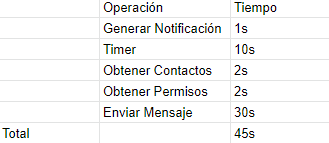
\includegraphics[width=.50\textwidth]{AvancesPruebas/imagenes/TNA}}
	\caption{Tiempos notificación automática}
	\label{fig:TNA}
\end{figure}

En la figura se muestra la tabla de tiempo para una notificación manual.

\begin{figure}[htbp!]
	\centering
	\fbox{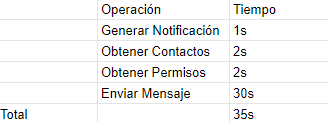
\includegraphics[width=.50\textwidth]{AvancesPruebas/imagenes/TNM}}
	\caption{Tiempos notificación manual}
	\label{fig:TNM}
\end{figure}

Las pruebas fueron realizadas en ambientes totalmente controlados, mismos que no tuvieron un inconvenientes con la comunicación de red para el envió de mensajes ni consultas a la BD, estos tiempos pudieran ser variables dependiendo las dificultades de red que llegaran a presentarse. Ademas se realizo el envío de notificaciones a una lista de 3 contactos, uno de cada tipo.





 